\documentclass[10pt,a4paper,english,italian]{article}
\usepackage[T1]{fontenc}
\usepackage[latin1]{inputenc}
\usepackage{babel}
\usepackage{color}
\usepackage{amssymb}
\usepackage{amsmath}
\usepackage{epsfig}
\usepackage{tabularx}
\usepackage{multirow}
\usepackage{subfigure}
\usepackage{babel}
\usepackage{verbatim}
\usepackage{fancyhdr}
\usepackage{psfrag}
\usepackage{listings}
\usepackage{../common/espacs}

\setlength{\textwidth}{100ex}
\setlength{\oddsidemargin}{0ex}

\pagestyle{fancy}
\headheight 35pt

\rhead{\copyright~Copyright 2006 Daniele A. Di Pietro}

\makeatother

\title{Esercitazione 2}
\author{D. A. Di Pietro}

\begin{document}
\lstset{language=[ISO]C++}
\maketitle 

Il calcolo degli autovalori di una matrice \`e richiesto in molte
applicazioni ingegneristiche: un esempio classico \`e l'analisi delle
frequenze naturali di sistemi fisici. I metodi numerici per il calcolo
degli autovettori si distinguono in \emph{parziali}, adatti al calcolo
degli autovalori estremi, e \emph{globali}, in grado di approssimare
l'intero spettro della matrice.

Il \emph{metodo delle potenze} \`e applicabile a matrici in cui
l'autovalore di modulo massimo $\lambda_1$ abbia molteplicit\`a
unitaria e sia ben separato dall'autovalore immediatamente pi\`u
piccolo in modulo. Il generico passo dell'algoritmo \`e riportato di
seguito:
\begin{equation*}
\begin{aligned}
{\bf q}\iter{k} &= \frac{ A{\bf q}\iter{k-1} }{ \norm{ A{\bf q}\iter{k-1}}_2 },\\
{\bf \nu}\iter{k} &= {{\bf q}\iter{k}}^T  A {\bf q}\iter{k},\\
{\bf w}\iter{k} &= \frac{ {\bf w}\iter{k-1}A }{ \norm{ {\bf w}\iter{k-1} A}_2 },
\end{aligned}
\end{equation*}
dove con $\nu\iter{k}$, ${\bf q}\iter{k}$ e ${\bf w}\iter{k}$ si sono
indicate, rispettivamente, le approssimazioni di $\lambda_1$ e degli
autovalori destro e sinistro ${\bf x}_1$ e ${\bf y}_1$ ad esso
associati. Vale la seguente stima, utile per determinare un criterio
d'arresto:
\begin{equation*}
\module{ \lambda_1 - \nu\iter{k} } \approx %
\frac{ \norm{ {\bf r}\iter{k} }_2 }{ \module{ {\bf w}\iter{k}\cdot{\bf q}\iter{k} } },
\end{equation*}
dove ${\bf r}\iter{k} \eqbydef A{\bf q}\iter{k} - \nu\iter{k}{\bf
q}\iter{k}$ \`e il residuo all'iterazione $k$-esima.

Il \emph{metodo di Jacobi} consente di approssimare l'intero spettro
di una matrice simmetrica. L'idea dell'algoritmo \`e quella di
ottenere, a partire da $A$, una matrice quasi diagonale
$A\iter{k}\approx D$ ortogonalmente simile ad $A$ che abbia sulla
diagonale principale le approssimazioni degli autovalori di $A$. La
$k$-esima iterazione richiede di fissare una coppia di indici
$\couple{p\iter{k}}{q\iter{k}}$ e costruire, a partire da
$A\iter{k-1}$, la successiva approssimazione $A\iter{k}$ in modo tale
che
\begin{equation}
a\iter{k}_{pq} = 0.
\label{eq:jacobi:cond}
\end{equation}
Tale approssimazione si calcola mediante una opportuna
\emph{trasformazione di Givens}:
\begin{equation*}
A\iter{k} = G(p\iter{k}, q\iter{k}, \theta\iter{k})^T %
A\iter{k-1} %
G(p\iter{k}, q\iter{k}, \theta\iter{k}),
\end{equation*}
dove l'angolo di rotazione $\theta\iter{k}$ \`e determinato in modo da
soddisfare la condizione \eqref{eq:jacobi:cond}. La matrice di Givens
\`e definita come
\begin{equation*}
\function{G}{i,k,\theta} = I_n - Y,
\end{equation*}
essendo $Y\in\mathbb{R}^{n\times n}$ una matrice nulla eccetto che per
i seguenti valori: $y_{ii} = y_{kk} = 1 - \cos\theta $ e $y_{ik} =
-y_{ki} = -\sin\theta$. Fissata la coppia di indici
$\couple{p\iter{k}}{q\iter{k}}$ relativa alla $k$-esima iterazione,
vale la seguente formula per il calcolo delle funzioni trigonometriche
dell'angolo di rotazione (per brevit\`a di notazione si omette l'apice
quando \`e pari a $k$):
\begin{equation*}
\couple{\cos\theta}{\sin\theta} = %
\begin{cases}
    \couple{1}{0} & \Se{a_{pq}\iter{k-1} = 0}, \\
    \couple{1 / \sqrt{1 + t^2}}{t / \sqrt{1 + t^2}} & \Altrimenti,
\end{cases}
\end{equation*}
dove, posto $\eta \eqbydef \left( a_{qq}\iter{k-1} -
a_{pp}\iter{k-1}\right)/{2a_{pq}\iter{k-1}}$:
\begin{equation*}
t = \begin{cases}
    1 / \left( \eta + \sqrt{1 + \eta^2}\right) & \Se{\eta\ge 0}, \\
    -1 / \left( -\eta + \sqrt{1 + \eta^2}\right) & \Altrimenti.
\end{cases}
\end{equation*}
La coppia di indici $\couple{p\iter{k}}{q\iter{k}}$ pu\`o essere
fissata scorrendo la matrice per riga e scegliendo in sucessione le
entrate nella parte strettamente triangolare superiore (metodo di
Jacobi \emph{ciclico}). Terminata una passata completa (\emph{sweep}),
si ricomincia dalla prima riga. Il metodo si arresta quando la
seguente condizione \`e soddisfatta:
\begin{equation*}
\frac{ \norm{ A\iter{k} - \diag{A\iter{k}} }_F }{ \norm{ A }_F } \le %
\mathtt{tol},
\end{equation*}
avendo indicato con $\norm{\cdot}_F$ la norma di Frobenius. Entrambi i
metodi sono descritti pi\`u dettagliatamente in
\cite[\extref{5}]{Quarteroni.Sacco.ea:2000}.

La codifica dei metodi per il calcolo degli autovalori di una matrice
richiede una libreria per la gestione dell'algebra
lineare. L'implementazione C++ proposta beneficia delle capacit� di
astrazione del linguaggio, che consente, mediante la definizione di
tipi utente ed il sovraccaricamento degli operatori, di utilizzare una
notazione che ricalca quella convenzionale. Come vedremo, bench� tale
soluzione appaia senz'altro elegante, pu� non essere la pi�
efficiente, poich� l'astrazione ha un costo computazionale. Inoltre,
esistono numerose librerie che implementano questi costrutti di base,
il cui utilizzo andrebbe considerato prima di scrivere codice specifico.

Si richiede di
\begin{enumerate}
\item prendendo come modello la soluzione proposta per il metodo di Jacobi ciclico, scrivere una classe che implementi il metodo delle potenze;
\item completare l'implementazione della libreria per l'algebra
lineare, aggiungendo la funzionalit� di prodotto matrice per vettore
(\cpp{operator*} per la classe \cpp{Matrix}) e vettore per matrice (\cpp{operator*} binario);
\item derivare una classe \cpp{Hilbert} dalla classe \cpp{Matrix};
\item \label{validazione} validare il codice utilizzandolo per calcolare gli autovalori
della matrice di Hilbert di dimensione $4$, il cui spettro \`e
riportato sotto fino alla quinta cifra significativa:
\begin{equation*}
\sigma\left( H_4\right) = %
\left\{
    1.5002, 1.6914\e{-1}, 6.7383\e{-3}, 9,6792\e{-5}
\right\}.
\end{equation*}
\item per lo svolgimento del punto \ref{validazione} utilizzare una libreria per l'algebra lineare diversa da quella proposta (ad esempio \cpp{ublas}): modificare (se necessario) il codice.
\end{enumerate}

\newpage

\section*{Soluzione}

La \emph{policy} per il parametro \cpp{template} \cpp{Preconditioner}
\`e la disponibilit\`a di un membro \cpp{solve} in grado di ricevere
un \cpp{Vector} e che restituisca un \cpp{Vector}. Una scelta naturale
\`e quindi la definizione di una classe \cpp{Preconditioner},
\cpp{template} rispetto al tipo del vettore.

Il pi\`u semplice precondizionatore \`e il precondizionatore
\emph{identit\`a}.

\lstset{basicstyle=\scriptsize\sf}
\lstinputlisting[caption=L'interfaccia della classe
\cpp{IdentityPrecond},
linerange={14-43}]{./es/src/solver_policies.hpp}
\lstset{basicstyle=\sf}

Un precondizionatore pi\`u complesso pu\`o essere costruito ricorrendo
a librerie di calcolo per il metodo \cpp{solve}, che fornisce la
soluzione del sistema lineare di precondizionamento. Si propone come
esempio un precondizionatore \emph{diagonale}, ottimale per matrice
simmetrica definita positiva \cite{Quarteroni.Sacco.ea:2000}: il solutore utilizzato \`e fornito dalla
libreria \cpp{boost} per sistemi triangolari.

\lstset{basicstyle=\scriptsize\sf}
\lstinputlisting[caption=L'interfaccia della classe
\cpp{UblasTriPrecond},
linerange={45-88}]{./es/src/solver_policies.hpp}
\lstset{basicstyle=\sf}

Si noti il parametro \cpp{template} \cpp{C} per la classe
\cpp{UblasTriPrecond}, posto per \emph{default} uguale a
\cpp{UBLAS::lower_tag}: si tratta di un parametro richiesto dal solver
\cpp{UBLAS::solve} per distinguere una matrice triangolare superiore
da una matrice triangolare inferiore (si veda \cite{UBLASweb}).

Il \emph{main program} \`e riportato di seguito. La lettura delle
matrici da file viene effettuata sfruttando i metodi disponibili per
la classe \cpp{string} della STL. Il sistema lineare \`e risolto con i
due diversi precondizionatori.

\lstset{basicstyle=\scriptsize\sf}
\lstinputlisting[caption=Il \emph{main program}]{./es/main.cpp}
\lstset{basicstyle=\sf}

Il risultato dell'esecuzione \`e il seguente:
\begin{verbatim}
Identity Preconditioner
        status = 0
        number of iterations = 10
        error = 2.78721e-19

Triangular Preconditioner
        status = 0
        number of iterations = 10
        error = 2.78721e-19
\end{verbatim}

Si noti che in questo esercizio l'effetto del precondizionatore diagonale non \`e decisivo
rispetto al caso di matrice non precondizionata (d'altra parte per il
caso in esame il precondizionatore diagonale \`e esattamente un
multiplo della matrice identit\`a).

Le \emph{performances} del codice possono essere
misurate con gli strumenti di analisi \emph{valgrind} e
\emph{gprof}. In particolare \`e interessante valutare l'occupazione di
memoria durante l'esecuzione del programma, in funzione del tipo di
strutture dati.
\begin{verbatim}
valgrind --tool=massif ./main
\end{verbatim}

\begin{figure}
\subfigure[Matrice piena]{
\centering
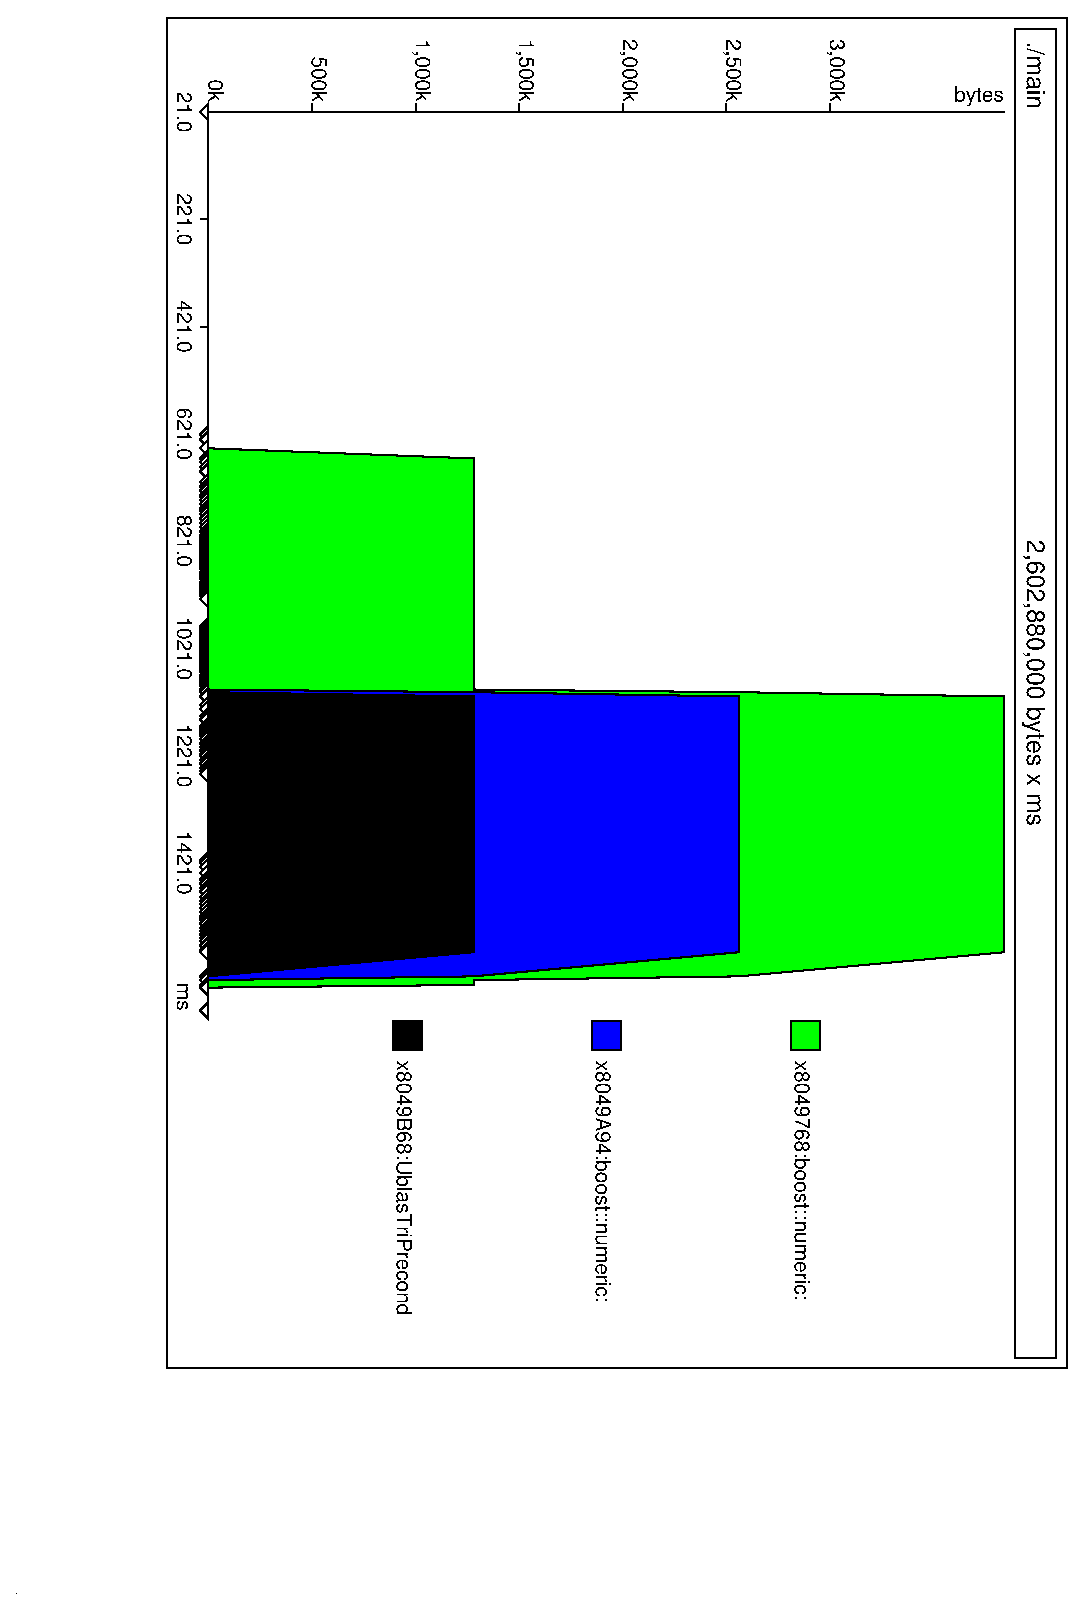
\includegraphics[height=.75\textwidth,angle=-270]{./massif.densebig.eps}
}
\subfigure[Matrice sparsa]{
\centering
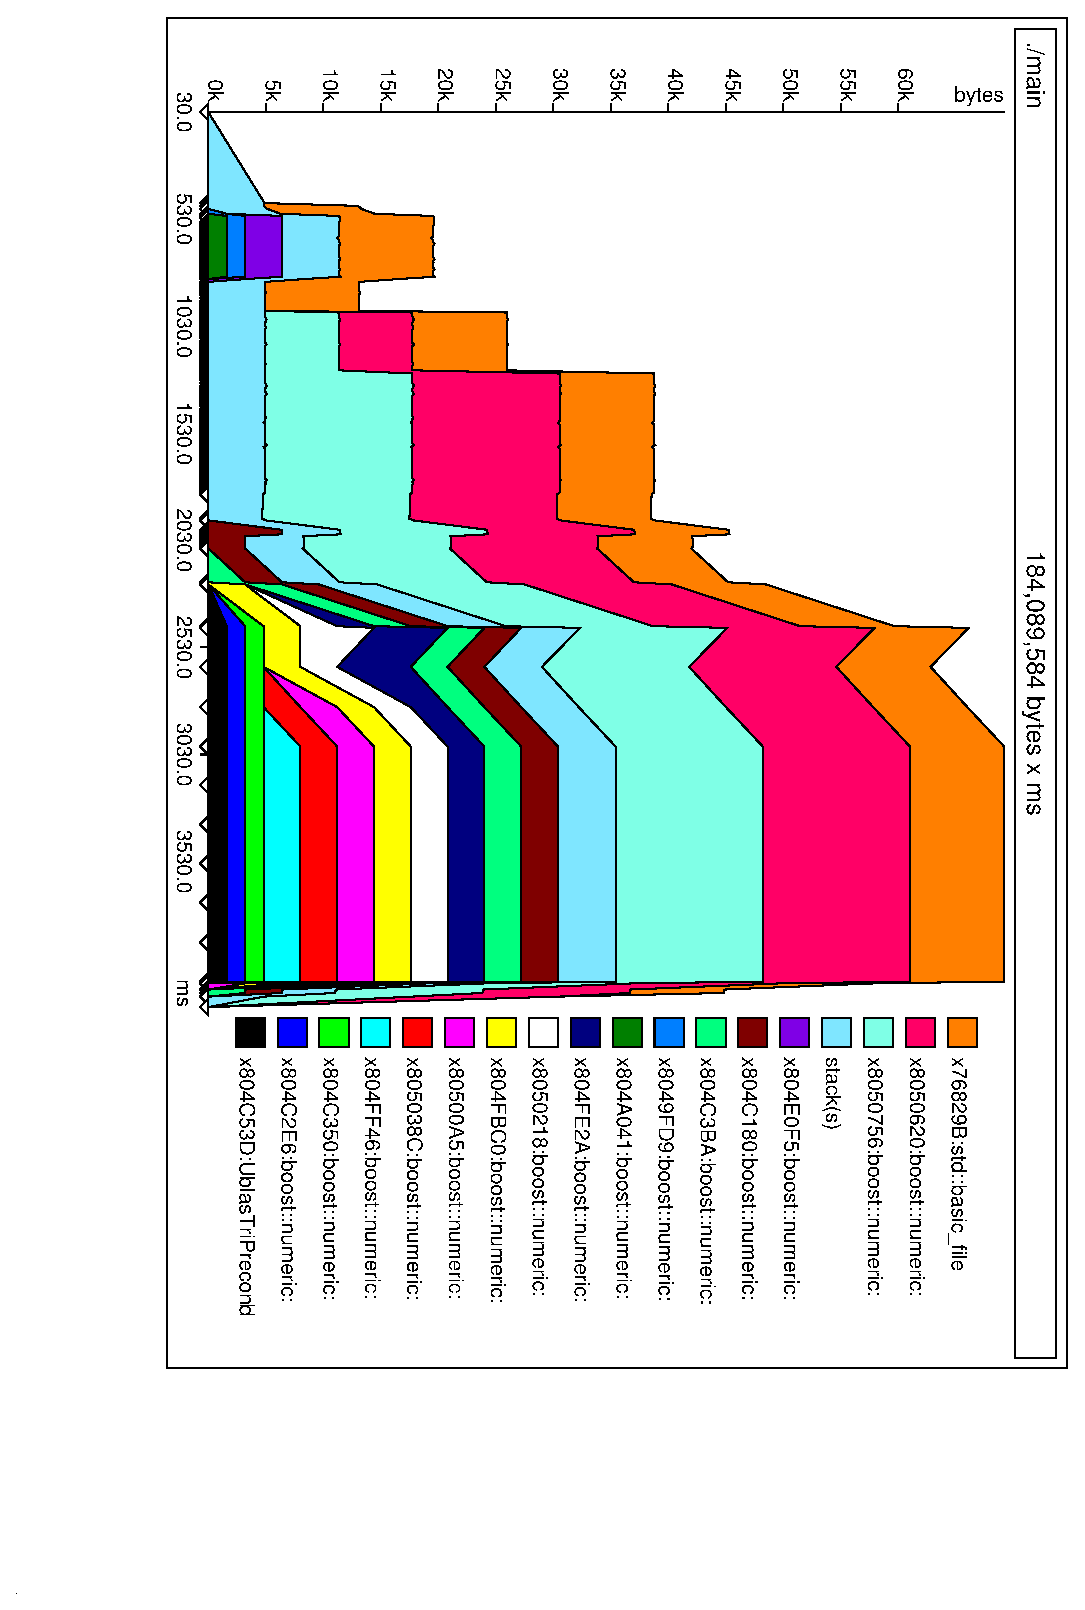
\includegraphics[height=.75\textwidth,angle=-270]{./massif.sparsebig.eps}
}
\caption{Occupazione di memoria durante l'esecuzione del programma,
  per la risoluzione di un sitema lineare quadrato di ordine 400.}
\label{fig:fin:results}
\end{figure}

I grafici generati da \texttt{valgrind} attraverso lo strumento
\texttt{massif} indicano dei valori di occupazione della memoria in
termini di \emph{spazio-tempo}: l'area sottesa alle curve misura
quanta memoria \emph{heap} \`e stata occupata, per quanto tempo. In effetti
il tempo di esecuzione del programma viene influenzato dalle
operazioni svolte da \texttt{valgrind}, quindi il dato pi\`u rilevante
\`e quello ``spaziale'' (in ordinata). In ciascun grafico si nota
quali operazioni del programma ne influenzino maggiormente le
prestazioni; confrontando i due grafici si ha un idea dell'effetto
dell'utilizzo dei due diversi formati di memorizzazione dei
dati. Informazioni dettagliate sulle misure realizzate da
\texttt{valgrind} sono riportate nel file di testo generato come
output. Per ottenere il maggior numero di indicazioni occorre
compilare il \emph{main program} con opzioni di \emph{debug}.

Si noti che, nell'implementazione proposta,
vengono utilizzati i tipi della libreria
\cpp{boost}: quando si utilizzano oggetti di tipo \cpp{matrix}, che
adottano il formato di memorizzazione pieno, l'occupazione della
memoria \`e decisamente pi\`u ingente. Il formato di memorizzazione sparso \`e adottato da
oggetti di tipo \cpp{coordinate_matrix}, grazie ai quali l'occupazione complessiva
di memoria \`e ridotta circa di un fattore 50 (nel caso di matrice
$400 \times 400$).




\bibliographystyle{siam}
\bibliography{../common/bibliography}

\end{document}
